\section{Trasformata Z}
La trasformata Z\citet{book:trasformataz}\index{Trasformata Z} permette di trasformare una funzione dal dominio del tempo discreto al dominio complesso discreto, ed è definita come segue:

\[ Z[x(i)]=X(z):=\sum_{i=-\infty}^{\infty}{x(i)\cdot z^{-i}},\quad z \in \mathbb{C}  \]

\noindent Vediamo due trasformate notevoli di cui faremo uso, ovvero, l'impulso (figura \ref{fig:impulsodiscreto}):

\[
x(i)=
\left\{
\begin{aligned}
1 \quad i=0 \\
0 \quad i\neq 0
\end{aligned}
\right.\Longrightarrow X(z)=1
\]

\begin{figure}[htbp]
  \centering
  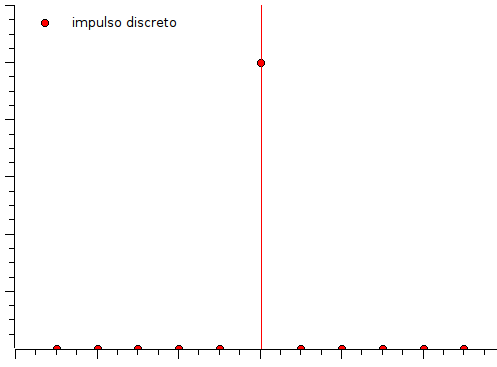
\includegraphics[scale=0.5]{img/impulsodiscreto.png}
  \caption{Impulso discreto\label{fig:impulsodiscreto}}
\end{figure}

\noindent e lo scalino (in figura \ref{fig:scalinodiscreto}):
\[
x(i)=
\left\{
\begin{aligned}
a \quad i\geq 0 \\
0 \quad i < 0
\end{aligned}
\right.\Longrightarrow X(z)=\frac{z}{z-a}
\]

\begin{figure}[htbp]
  \centering
  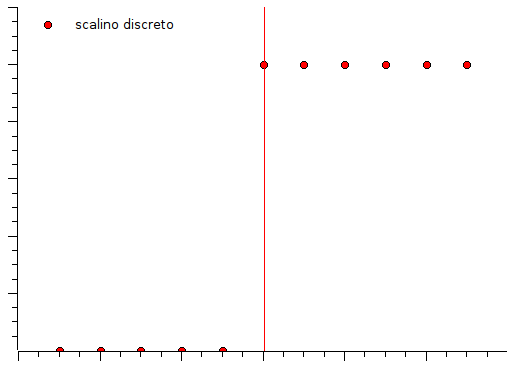
\includegraphics[scale=0.5]{img/scalinodiscreto.png}
  \caption{Scalino discreto\label{fig:scalinodiscreto}}
\end{figure}


La trasformata Z che consideriamo è sempre bilatera, ovvero esiste sia per posizioni negative che positive. Una funzione monolatera, di contro, esiste solo per i positivi.\newline
L'operazione di antitrasformazione è possibile ma è di uso poco pratico quindi non viene quasi mai utilizzata.
% ########################################################################
\subsection{Proprietà}
\paragraph{Proprietà 1 - Linearità} Se $x(i)$ e $y(i)$ sono due funzioni sugli interi con trasformata Zeta data rispettivamente da $X(z)$ e $Y(z)$, si ha che, qualunque siano le costanti $a$ e $b$:

  \[ Z[a\cdot x(i)+b\cdot y(i)]=a \cdot Z[x(i)] + b \cdot Z[y(i)]=aX(z)+bY(z) \]
  
con dominio che include o è uguale all'intersezione dei domini di $X(z)$ e $Y(z)$
\paragraph{Proprietà 2 - Traslazione} Se $x(i)$ è una funzione sugli interi con trasformata $X(z)$ e se $n_0 \in Z$ si ha:

  \[ Z[x(i-k)]=z^k\cdot Z[x(i)]=z^k\cdot X(z) \]
  
con dominio uguale al dominio di $X(z)$
\paragraph{Proprietà 3- Moltiplicazione per $i$} Se $x(i)$ è una funzione sugli interi con trasformata $X(z)$ allora:

  \[ Z[i \cdot x(i)]=-z\frac{dX(z)}{dz} \]
  
con dominio dato dalla stessa corona circolare di convergenza di $X(z)$
\paragraph{Proprietà 4 - Convoluzione} Se $x(i)$ e $y(i)$ sono due funzioni sugli interi con trasformata Zeta data rispettivamente da $X(z)$ e $Y(z)$ e se $x(i)$ e $y(i)$ hanno prodotto di convoluzione $x(i) \ast y(i) = \sum_{j=-\infty}^{\infty} {x(j)y(i-j)} = \sum_{j=-\infty}^{\infty} {x(i-j)y(j)}$, si ha che:

  \[ Z[x(i)\ast y(i)]=Z[x(i)]\ast Z[y(i)]=X(z)Y(z) \]
  
con dominio che include o è uguale all'intersezione dei domini di $x(z)$ e di $Y(z)$
% ########################################################################
\subsection{Confronto con Fourier}
Esiste una relazione fra la trasformata Z e la trasformata di Fourier\index{Trasformata di Fourier}. Sia $x(i)$ tale che $\sum_{i=-\infty}^{\infty} {|x(i)|}<\infty$\footnote{ovvero converge a zero velocemente}, allora esiste la trasformata di Fourier:

  \[ F[x(t)]=\sum_{t=-\infty}^{\infty}{x(t)e^{-j\omega t}}=\sum_{t=-\infty}^{\infty}{x(t)z^{-t}}, \quad j=\sqrt{-1},e^{j\omega}=z \]
  
\noindent e inoltre:

  \[ F(x(t))=X(e^{j\omega}) \]
  
%GRAFICHETTI
\paragraph{Osservazione 1} La trasformata Z è una funzione complessa di variabile complessa, mentre la trasformata di Fourier è una funzione complessa di variabile reale
\paragraph{Osservazione 2} L'antitrasformazione con la trasformata di Fourier è più semplice
